% Chapter I. Introduction


\section*{Mathematical Definitions and Examples}

\subsection*{1. Normal Subgroup}

\textbf{Definition:}

A subgroup \(N\) of a group \(G\) is called a \emph{normal subgroup} if it is invariant under conjugation, that is, for every element \(g \in G\) and \(n \in N\), the element \(gng^{-1} \in N\).

Symbolically:
\[ N \triangleleft G \iff \forall g \in G, \forall n \in N, \ gng^{-1} \in N. \]
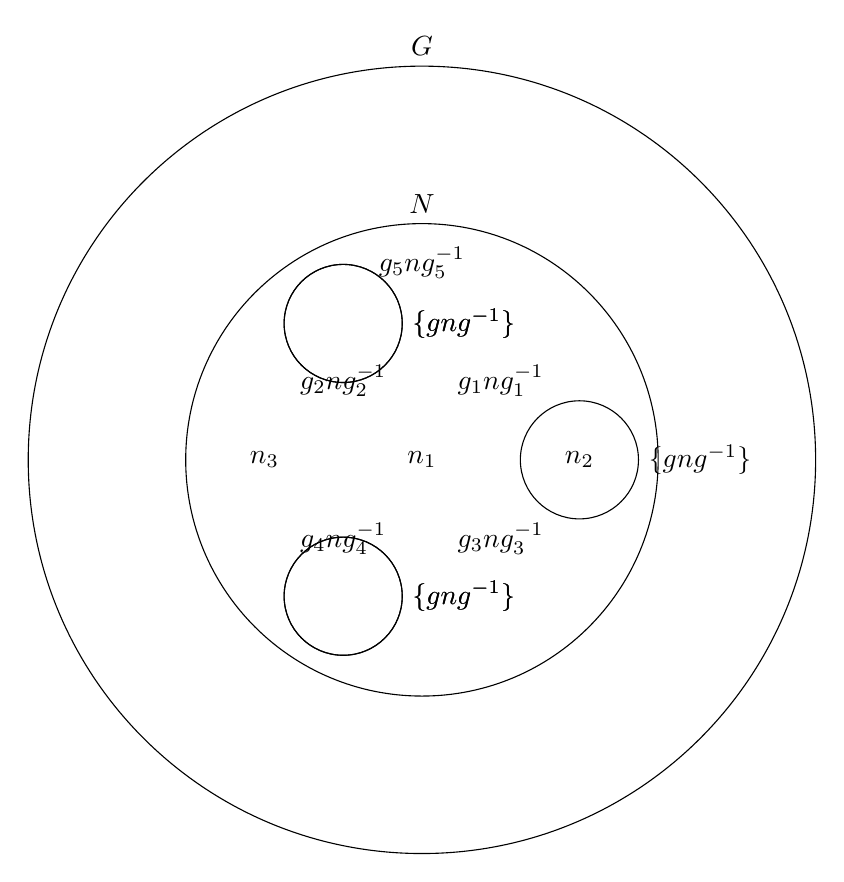
\begin{tikzpicture}
	% Draw the group G
	\node[draw, circle, minimum size=10cm, label=above:$G$] (G) at (0,0) {};
	
	% Draw the normal subgroup N inside G
	\node[draw, circle, minimum size=6cm, label=above:$N$] (N) at (0,0) {};
	
	% Draw conjugate sets inside N
	\foreach \i in {1,...,5} {
		\node[draw, circle, minimum size=1.5cm, label=right:$\{gng^{-1}\}$] at ({120*\i}:2) {};
	}
	
	% Labels for elements
	\node at (0,0) {$n_1$};
	\node at (2,0) {$n_2$};
	\node at (-2,0) {$n_3$};
	\node at (1,1) {$g_1ng_1^{-1}$};
	\node at (-1,1) {$g_2ng_2^{-1}$};
	\node at (1,-1) {$g_3ng_3^{-1}$};
	\node at (-1,-1) {$g_4ng_4^{-1}$};
	\node at (0,2.5) {$g_5ng_5^{-1}$};
\end{tikzpicture}

\textbf{Examples:}

1. In the group of integers \((\mathbb{Z}, +)\), the subgroup \(2\mathbb{Z} = \{2k \mid k \in \mathbb{Z}\}\) is a normal subgroup since \(\mathbb{Z}\) is abelian.
\[ 2\mathbb{Z} = \{2k \mid k \in \mathbb{Z}\} \triangleleft \mathbb{Z} \]
\begin{tikzpicture}
	% Draw the group Z
	\node[draw, circle, minimum size=6cm] (Z) at (0,0) {$\mathbb{Z}$};
	
	% Draw the normal subgroup 2Z inside Z
	\node[draw, circle, minimum size=3cm] (2Z) at (0,0) {$2\mathbb{Z}$};
	
	% Labels for elements
	\node at (2,1) {1};
	\node at (3,2) {2};
	\node at (4,0) {3};
	\node at (2,-2) {4};
	\node at (-2,-1) {-1};
	\node at (-3,-2) {-2};
	\node at (-4,0) {-3};
	\node at (-2,2) {-4};
\end{tikzpicture}
2. In the symmetric group \(S_3\), the subgroup \(A_3 = \{(1), (123), (132)\}\) (the alternating group) is a normal subgroup.
\[ A_3 = \{(1), (123), (132)\} \triangleleft S_3 \]

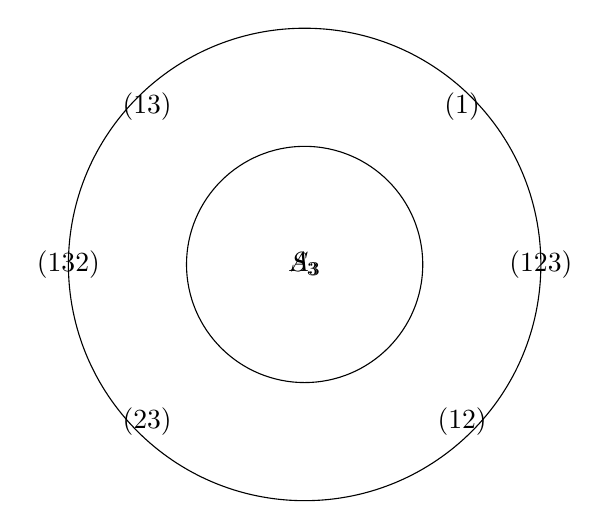
\begin{tikzpicture}
	% Draw the group S3
	\node[draw, circle, minimum size=6cm] (S3) at (0,0) {$S_3$};
	
	% Draw the normal subgroup A3 inside S3
	\node[draw, circle, minimum size=3cm] (A3) at (0,0) {$A_3$};
	
	% Labels for elements of S3
	\node at (2,2) {$(1)$};
	\node at (2,-2) {$(12)$};
	\node at (-2,2) {$(13)$};
	\node at (-2,-2) {$(23)$};
	\node at (3,0) {$(123)$};
	\node at (-3,0) {$(132)$};
\end{tikzpicture}
\subsection*{2. Quotient Group (Factor Group)}

\textbf{Definition:}

Given a group \(G\) and a normal subgroup \(N\) of \(G\), the \emph{quotient group} (or \emph{factor group}) \(G/N\) is the set of left cosets of \(N\) in \(G\) with the group operation defined by:
\[ (gN) \cdot (hN) = (gh)N \]

\textbf{Examples:}

1. For \((\mathbb{Z}, +)\) and \(N = 2\mathbb{Z}\), the quotient group \(\mathbb{Z}/2\mathbb{Z}\) consists of two cosets: \(0 + 2\mathbb{Z}\) and \(1 + 2\mathbb{Z}\).
\[ \mathbb{Z}/2\mathbb{Z} = \{0 + 2\mathbb{Z}, 1 + 2\mathbb{Z}\} \]

\begin{tikzpicture}
	% Draw the group Z
	\node[draw, circle, minimum size=10cm, label=above:$\mathbb{Z}$] (Z) at (0,0) {};
	
	% Draw the cosets
	\node[draw, ellipse, minimum width=8cm, minimum height=3cm, label=above:$0 + 2\mathbb{Z}$] (even) at (0,2) {};
	\node[draw, ellipse, minimum width=8cm, minimum height=3cm, label=below:$1 + 2\mathbb{Z}$] (odd) at (0,-2) {};
	
	% Labels for elements
	\node at (0,2) {0};
	\node at (2,2) {2};
	\node at (-2,2) {-2};
	\node at (4,2) {4};
	\node at (-4,2) {-4};
	
	\node at (0,-2) {1};
	\node at (2,-2) {3};
	\node at (-2,-2) {-1};
	\node at (4,-2) {5};
	\node at (-4,-2) {-3};
\end{tikzpicture}

2. In \(S_3\), the quotient group \(S_3/A_3\) is isomorphic to \(\mathbb{Z}_2\).
\[ S_3/A_3 \cong \mathbb{Z}_2 \]

\begin{tikzpicture}
	% Draw the group S3
	\node[draw, circle, minimum size=10cm, label=above:$S_3$] (S3) at (0,0) {};
	
	% Draw the normal subgroup A3 inside S3
	\node[draw, circle, minimum size=4cm, label=above:$A_3$] (A3) at (0,2) {};
	
	% Draw the coset containing elements not in A3
	\node[draw, ellipse, minimum width=6cm, minimum height=2cm, label=below:$S_3 \setminus A_3$] (notA3) at (0,-2) {};
	
	% Labels for elements of A3
	\node at (0,2) {$(1)$};
	\node at (2,2) {$(123)$};
	\node at (-2,2) {$(132)$};
	
	% Labels for elements of S3 not in A3
	\node at (0,-2) {$(12)$};
	\node at (2,-2) {$(13)$};
	\node at (-2,-2) {$(23)$};
\end{tikzpicture}

\subsection*{3. Ring}

\textbf{Definition:}

A \emph{ring} is a set \(R\) equipped with two binary operations \(+\) and \(\cdot\) (addition and multiplication) such that:
\begin{enumerate}
	\item \((R, +)\) is an abelian group.
	\item \((R, \cdot)\) is a monoid.
	\item Multiplication is distributive over addition: for all \(a, b, c \in R\), \(a \cdot (b + c) = a \cdot b + a \cdot c\) and \((a + b) \cdot c = a \cdot c + b \cdot c\).
\end{enumerate}

\textbf{Examples:}

1. The set of integers \(\mathbb{Z}\) with usual addition and multiplication.
\[ \mathbb{Z} \text{ is a ring} \]

\begin{tikzpicture}
	% Draw the integers as points on a number line
	\foreach \x in {-4, -3, -2, -1, 0, 1, 2, 3, 4} {
		\node[circle, draw, fill=white] at (\x, 0) {};
		\node[below] at (\x, 0) {\x};
	}
	
	% Addition example: 1 + 2 = 3
	\draw[->, thick] (1, 0.2) to[out=60, in=120] (2, 0.2);
	\node[above] at (1.5, 1) {+};
	\draw[->, thick] (2, 0.2) to[out=60, in=120] (3, 0.2);
	\node[above] at (2.5, 1) {=};
	\node[above] at (3, 1.2) {3};
	
	% Multiplication example: 2 * 2 = 4
	\draw[->, thick, red] (2, -0.2) to[out=-60, in=-120] (2, -0.2);
	\node[below, red] at (2, -1.2) {\(\cdot\)};
	\draw[->, thick, red] (2, -0.2) to[out=-60, in=-120] (4, -0.2);
	\node[below, red] at (4, -1.2) {=};
	\node[below, red] at (4, -1.5) {4};
\end{tikzpicture}

2. The set of \(2 \times 2\) matrices over \(\mathbb{R}\), \(M_2(\mathbb{R})\), with matrix addition and multiplication.
\[ M_2(\mathbb{R}) \text{ is a ring} \]
\begin{tikzpicture}
	% Matrix A
	\matrix[matrix of math nodes,left delimiter=(,right delimiter=)] (A) at (0,0)
	{ 1 & 2 \\ 3 & 4 \\ };
	
	% Plus sign
	\node at (2,0) {+};
	
	% Matrix B
	\matrix[matrix of math nodes,left delimiter=(,right delimiter=)] (B) at (4,0)
	{ 5 & 6 \\ 7 & 8 \\ };
	
	% Equals sign
	\node at (6,0) {=};
	
	% Matrix C (A + B)
	\matrix[matrix of math nodes,left delimiter=(,right delimiter=)] (C) at (8,0)
	{ 6 & 8 \\ 10 & 12 \\ };
	
	% Matrix A (again, for multiplication example)
	\matrix[matrix of math nodes,left delimiter=(,right delimiter=)] (A2) at (0,-3)
	{ 1 & 2 \\ 3 & 4 \\ };
	
	% Multiplication sign
	\node at (2,-3) {$\cdot$};
	
	% Matrix B (again, for multiplication example)
	\matrix[matrix of math nodes,left delimiter=(,right delimiter=)] (B2) at (4,-3)
	{ 5 & 6 \\ 7 & 8 \\ };
	
	% Equals sign
	\node at (6,-3) {=};
	
	% Matrix D (A * B)
	\matrix[matrix of math nodes,left delimiter=(,right delimiter=)] (D) at (8,-3)
	{ 19 & 22 \\ 43 & 50 \\ };
\end{tikzpicture}

\subsection*{4. Ideal}

\textbf{Definition:}

An \emph{ideal} \(I\) of a ring \(R\) is a subset of \(R\) such that:
\begin{enumerate}
	\item \(I\) is an additive subgroup of \(R\).
	\item For every \(r \in R\) and \(i \in I\), both \(ri\) and \(ir\) are in \(I\).
\end{enumerate}

\textbf{Examples:}

1. In \(\mathbb{Z}\), the set \(2\mathbb{Z}\) (all even integers) is an ideal.
\[ 2\mathbb{Z} = \{2k \mid k \in \mathbb{Z}\} \text{ is an ideal of } \mathbb{Z} \]
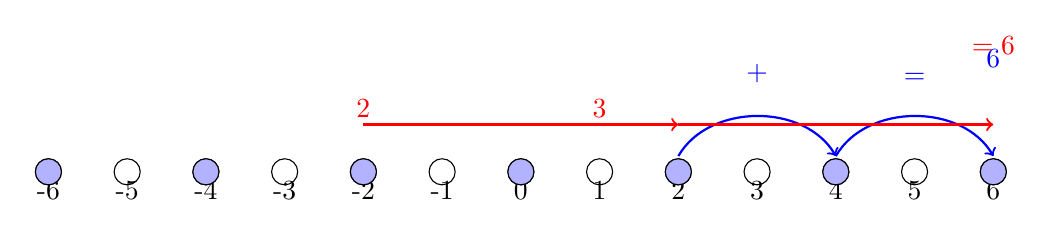
\begin{tikzpicture}
	% Draw the integers as points on a number line
	\foreach \x in {-6, -5, -4, -3, -2, -1, 0, 1, 2, 3, 4, 5, 6} {
		\node[circle, draw, fill=white] at (\x, 0) {};
		\node[below] at (\x, 0) {\x};
	}
	
	% Highlight the even integers
	\foreach \x in {-6, -4, -2, 0, 2, 4, 6} {
		\node[circle, draw, fill=blue!30] at (\x, 0) {};
	}
	
	% Addition example: 2 + 4 = 6
	\draw[->, thick, blue] (2, 0.2) to[out=60, in=120] (4, 0.2);
	\node[above, blue] at (3, 1) {+};
	\draw[->, thick, blue] (4, 0.2) to[out=60, in=120] (6, 0.2);
	\node[above, blue] at (5, 1) {=};
	\node[above, blue] at (6, 1.2) {6};
	
	% Multiplication example: 2 * 3 = 6
	\node[red] at (-2, 0.8) {$2$};
	\node[red] at (1, 0.8) {$3$};
	\node[red] at (6, 1.6) {$= 6$};
	\draw[->, thick, red] (-2, 0.6) -- (0, 0.6) -- (2, 0.6);
	\draw[->, thick, red] (2, 0.6) -- (4, 0.6) -- (6, 0.6);
\end{tikzpicture}
2. In the ring \(\mathbb{R}[x]\), the set of polynomials divisible by \(x\), denoted by \((x)\), is an ideal.
\[ (x) = \{x \cdot f(x) \mid f(x) \in \mathbb{R}[x]\} \text{ is an ideal of } \mathbb{R}[x] \]
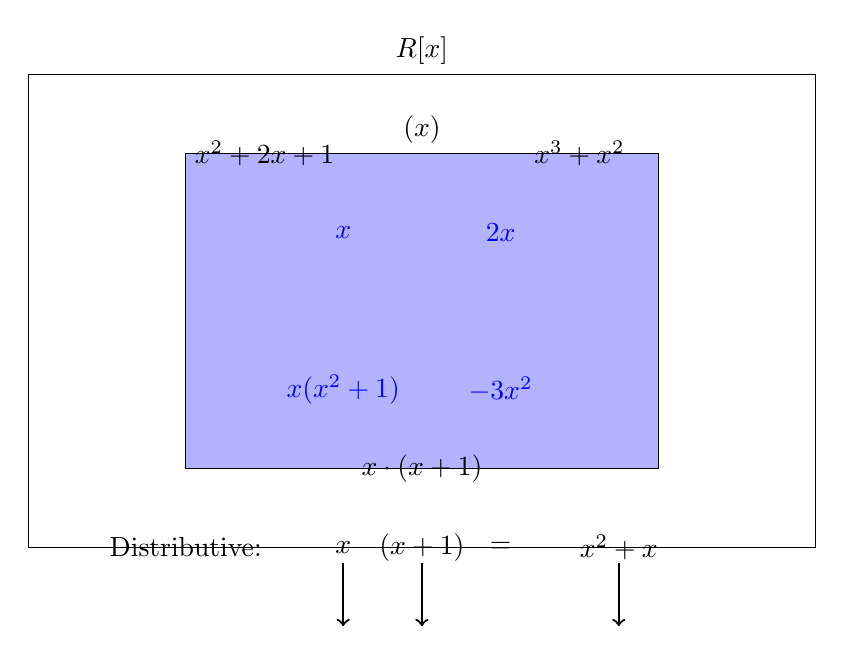
\begin{tikzpicture}
	% Draw the set of polynomials
	\node[draw, rectangle, minimum width=10cm, minimum height=6cm, label=above:{$\mathbb{R}[x]$}] (R) at (0,0) {};
	
	% Draw the ideal (x)
	\node[draw, rectangle, fill=blue!30, minimum width=6cm, minimum height=4cm, label=above:$(x)$] (I) at (0,0) {};
	
	% Examples of polynomials
	\node at (-2, 2) {$x^2 + 2x + 1$};
	\node at (2, 2) {$x^3 + x^2$};
	\node at (0, -2) {$x \cdot (x+1)$};
	
	% Examples of polynomials in (x)
	\node[blue] at (-1, 1) {$x$};
	\node[blue] at (1, 1) {$2x$};
	\node[blue] at (-1, -1) {$x(x^2 + 1)$};
	\node[blue] at (1, -1) {$-3x^2$};
	
	% Distributive example: x * (x+1) = x^2 + x
	\node at (-3, -3) {Distributive:};
	\node at (-1, -3) {$x$};
	\node at (0, -3) {$(x + 1)$};
	\node at (1, -3) {$=$};
	\node at (2.5, -3) {$x^2 + x$};
	
	\draw[->, thick] (-1, -3.2) -- (-1, -4);
	\draw[->, thick] (0, -3.2) -- (0, -4);
	\draw[->, thick] (2.5, -3.2) -- (2.5, -4);
	
\end{tikzpicture}
\subsection*{5. Prime Ideal}

\textbf{Definition:}

An ideal \(P\) in a ring \(R\) is a \emph{prime ideal} if \(P \neq R\) and whenever \(a \cdot b \in P\) for \(a, b \in R\), then \(a \in P\) or \(b \in P\).

\textbf{Examples:}

1. In \(\mathbb{Z}\), the ideal \( (p) \) where \(p\) is a prime number (e.g., \((5)\)) is a prime ideal.
\[ (5) = \{5k \mid k \in \mathbb{Z}\} \text{ is a prime ideal of } \mathbb{Z} \]

\begin{center}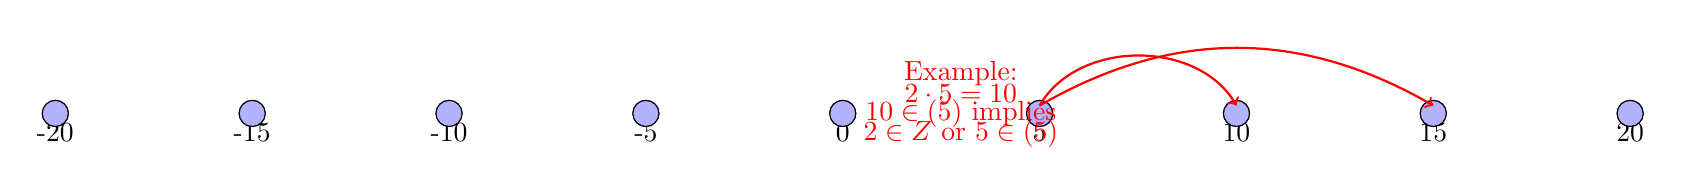
\begin{tikzpicture}[scale=.5]
		% Draw the integers as points on a number line
		\foreach \x in {-20, -15, -10, -5, 0, 5, 10, 15, 20} {
			\node[circle, draw, fill=white] at (\x, 0) {};
			\node[below] at (\x, 0) {\x};
		}
		
		% Highlight the multiples of 5
		\foreach \x in {-20, -15, -10, -5, 0, 5, 10, 15, 20} {
			\node[circle, draw, fill=blue!30] at (\x, 0) {};
		}
		
		% Illustrate the property: if a*b in (5), then a or b in (5)
		\node[red] at (3, 1) {Example:};
		\node[red] at (3, 0.5) {$2 \cdot 5 = 10$};
		\node[red] at (3, 0) {$10 \in (5)$ implies};
		\node[red] at (3, -0.5) {$2 \in \mathbb{Z}$ or $5 \in (5)$};
		
		% Lines to indicate the multiplication example
		\draw[->, thick, red] (5, 0.2) to[out=60, in=120] (10, 0.2);
		\draw[->, thick, red] (5, 0.2) to[out=30, in=150] (15, 0.2);
	\end{tikzpicture}
\end{center}

2. In \(\mathbb{Z}[x]\), the ideal \((x)\) is a prime ideal.
\[ (x) = \{x \cdot f(x) \mid f(x) \in \mathbb{Z}[x]\} \text{ is a prime ideal of } \mathbb{Z}[x] \]

\begin{center}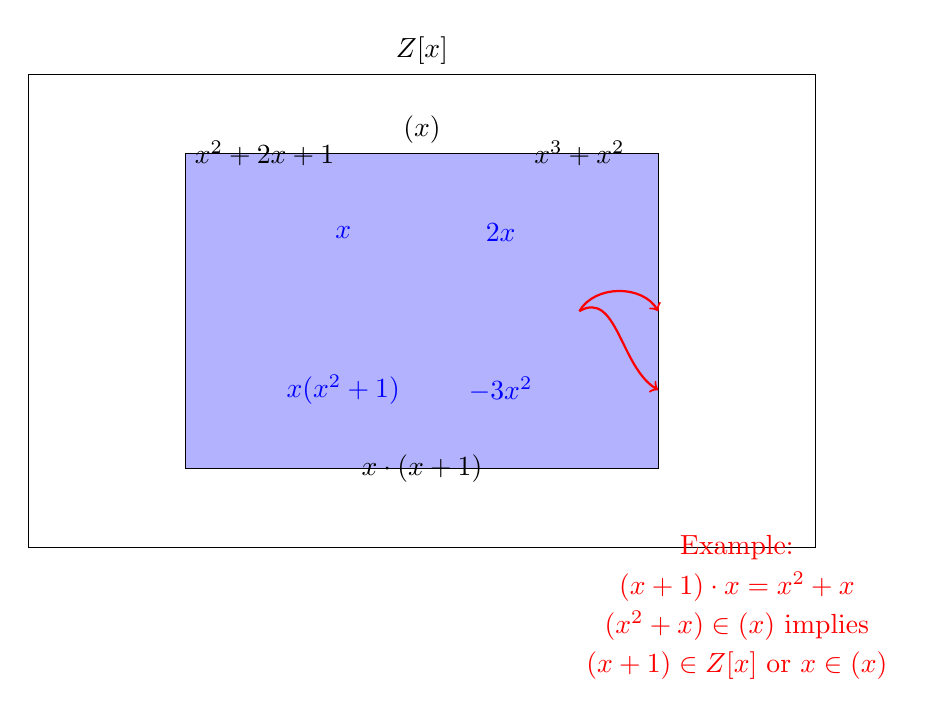
\begin{tikzpicture}
		% Draw the set of polynomials
		\node[draw, rectangle, minimum width=10cm, minimum height=6cm, label=above:{$\mathbb{Z}[x]$}] (R) at (0,0) {};
		
		% Draw the ideal (x)
		\node[draw, rectangle, fill=blue!30, minimum width=6cm, minimum height=4cm, label=above:$(x)$] (I) at (0,0) {};
		
		% Examples of polynomials
		\node at (-2, 2) {$x^2 + 2x + 1$};
		\node at (2, 2) {$x^3 + x^2$};
		\node at (0, -2) {$x \cdot (x+1)$};
		
		% Examples of polynomials in (x)
		\node[blue] at (-1, 1) {$x$};
		\node[blue] at (1, 1) {$2x$};
		\node[blue] at (-1, -1) {$x(x^2 + 1)$};
		\node[blue] at (1, -1) {$-3x^2$};
		
		% Illustrate the property: if a*b in (x), then a or b in (x)
		\node[red] at (4, -3) {Example:};
		\node[red] at (4, -3.5) {$(x+1) \cdot x = x^2 + x$};
		\node[red] at (4, -4) {$(x^2 + x) \in (x)$ implies};
		\node[red] at (4, -4.5) {$(x+1) \in \mathbb{Z}[x]$ or $x \in (x)$};
		
		% Arrows to indicate the multiplication example
		\draw[->, thick, red] (2, 0) to[out=30, in=150] (3, -1);
		\draw[->, thick, red] (2, 0) to[out=60, in=120] (3, 0);
	\end{tikzpicture}
\end{center}

\subsection*{6. Maximal Ideal}

\textbf{Definition:}

An ideal \(M\) in a ring \(R\) is a \emph{maximal ideal} if \(M \neq R\) and there are no other ideals \(I\) such that \(M \subset I \subset R\).

\textbf{Examples:}

1. In \(\mathbb{Z}\), the ideal \((p)\) where \(p\) is a prime number (e.g., \((3)\)) is a maximal ideal.
\[ (3) = \{3k \mid k \in \mathbb{Z}\} \text{ is a maximal ideal of } \mathbb{Z} \]

\begin{center}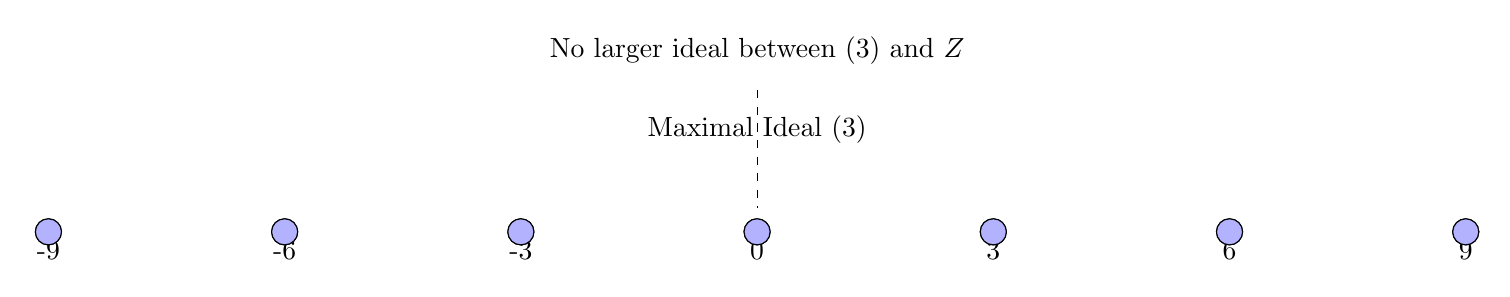
\begin{tikzpicture}
		% Draw the integers as points on a number line
		\foreach \x in {-9, -6, -3, 0, 3, 6, 9} {
			\node[circle, draw, fill=white] at (\x, 0) {};
			\node[below] at (\x, 0) {\x};
		}
		
		% Highlight the multiples of 3
		\foreach \x in {-9, -6, -3, 0, 3, 6, 9} {
			\node[circle, draw, fill=blue!30] at (\x, 0) {};
		}
		
		% Text for maximal ideal
		\node[above] at (0, 1) {Maximal Ideal $(3)$};
		\node[above] at (0, 2) {No larger ideal between $(3)$ and $\mathbb{Z}$};
		
		% Indicating no intermediate ideal
		\draw[dashed] (0, 1.8) -- (0, 0.3);
	\end{tikzpicture}
\end{center}

2. In \(\mathbb{R}[x]\), the ideal \((x - a)\) where \(a \in \mathbb{R}\) is a maximal ideal.
\[ (x - a) = \{(x - a) \cdot f(x) \mid f(x) \in \mathbb{R}[x]\} \text{ is a maximal ideal of } \mathbb{R}[x] \]

\begin{center}
	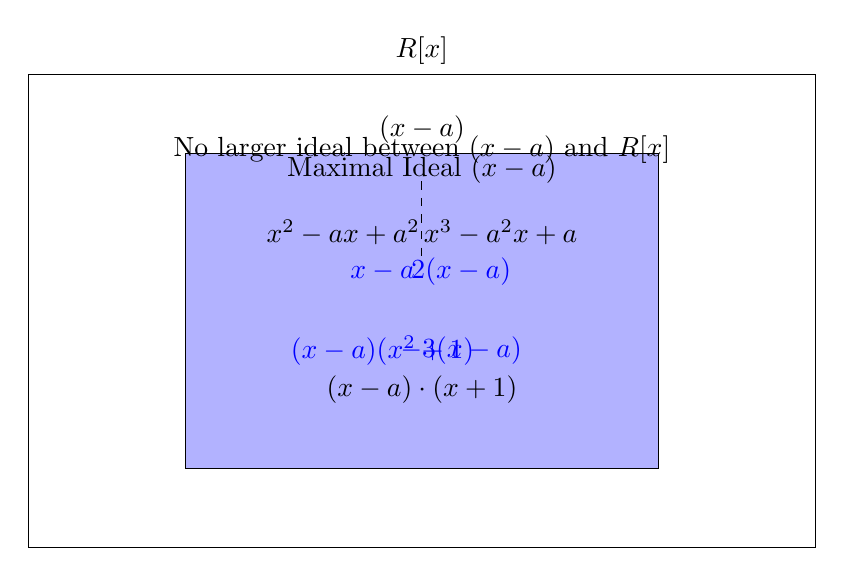
\begin{tikzpicture}[scale=.5]
		% Draw the set of polynomials
		\node[draw, rectangle, minimum width=10cm, minimum height=6cm, label=above:{$\mathbb{R}[x]$}] (R) at (0,0) {};
		
		% Draw the ideal (x - a)
		\node[draw, rectangle, fill=blue!30, minimum width=6cm, minimum height=4cm, label=above:$(x - a)$] (I) at (0,0) {};
		
		% Examples of polynomials
		\node at (-2, 2) {$x^2 - ax + a^2$};
		\node at (2, 2) {$x^3 - a^2x + a$};
		\node at (0, -2) {$(x - a) \cdot (x + 1)$};
		
		% Examples of polynomials in (x - a)
		\node[blue] at (-1, 1) {$x - a$};
		\node[blue] at (1, 1) {$2(x - a)$};
		\node[blue] at (-1, -1) {$(x - a)(x^2 + 1)$};
		\node[blue] at (1, -1) {$-3(x - a)$};
		
		% Text for maximal ideal
		\node[above] at (0, 3) {Maximal Ideal $(x - a)$};
		\node[above] at (0, 3.5) {No larger ideal between $(x - a)$ and $\mathbb{R}[x]$};
		
		% Indicating no intermediate ideal
		\draw[dashed] (0, 3.3) -- (0, 1.3);
		
	\end{tikzpicture}
\end{center}

\begin{tikzpicture}
	% Draw the set of 2x2 matrices
	\node[draw, rectangle, minimum width=10cm, minimum height=6cm, label=above:{$\text{M}_2(F)$}] (M2F) at (0,0) {};
	
	% Draw the GL(2, F) inside M2F
	\node[draw, rectangle, fill=blue!30, minimum width=6cm, minimum height=4cm, label=above:{$\text{GL}(2, F)$}] (GL2F) at (0,0) {};
	
	% Examples of matrices in GL(2, F)
	\node at (-1.5, 1.5) {$\begin{pmatrix} a & b \\ c & d \end{pmatrix}$};
	\node at (1.5, 1.5) {$\begin{pmatrix} 1 & 0 \\ 0 & 1 \end{pmatrix}$};
	\node at (0, -1) {$\begin{pmatrix} 2 & 1 \\ 3 & 4 \end{pmatrix}$};
	\node at (-1.5, -1.5) {Det $\neq 0$};
	
	% Examples of matrices not in GL(2, F)
	\node[red] at (4, 1) {$\begin{pmatrix} 1 & 2 \\ 2 & 4 \end{pmatrix}$};
	\node[red] at (4, -1) {$\begin{pmatrix} 0 & 0 \\ 0 & 0 \end{pmatrix}$};
	
	% Labels for examples
	\node at (-3, 2.5) {Examples in $\text{GL}(2, F)$};
	\node[red] at (4, 2.5) {Examples not in $\text{GL}(2, F)$};
\end{tikzpicture}


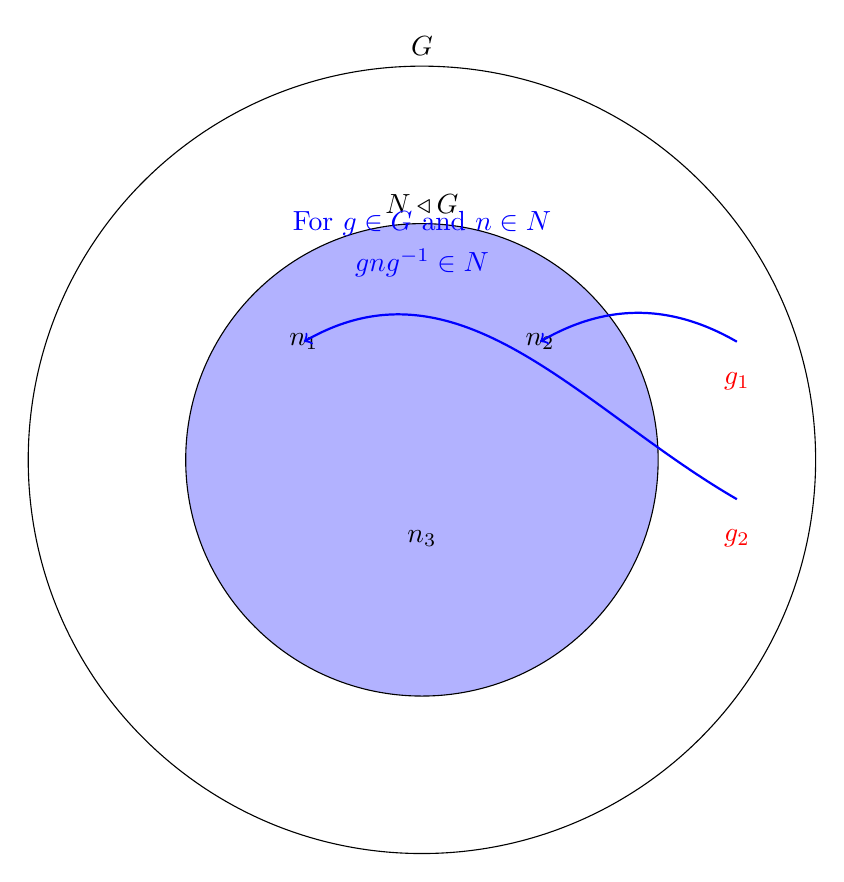
\begin{tikzpicture}
	% Draw the group G
	\node[draw, circle, minimum size=10cm, label=above:$G$] (G) at (0,0) {};
	
	% Draw the normal subgroup N inside G
	\node[draw, circle, fill=blue!30, minimum size=6cm, label=above:$N \triangleleft G$] (N) at (0,0) {};
	
	% Examples of elements in N
	\node at (-1.5, 1.5) {$n_1$};
	\node at (1.5, 1.5) {$n_2$};
	\node at (0, -1) {$n_3$};
	
	% Examples of elements in G but not in N
	\node[red] at (4, 1) {$g_1$};
	\node[red] at (4, -1) {$g_2$};
	
	% Illustration of normality
	\node[blue] at (0, 3) {For $g \in G$ and $n \in N$};
	\node[blue] at (0, 2.5) {$gng^{-1} \in N$};
	
	% Arrows for illustration
	\draw[->, thick, blue] (4, 1.5) to[out=150, in=30] (1.5, 1.5);
	\draw[->, thick, blue] (4, -0.5) to[out=150, in=30] (-1.5, 1.5);
\end{tikzpicture}

